\chapter{CAT(0)-Räume} % (fold)
\label{cha:1}

\begin{definition}[Metrischer Raum]
\label{def:1.1}
	Sei $X$ eine Menge.\marginnote{21.10.15 \\ \ [1]}
	Eine Abbildung $d \colon X \times X \rightarrow \RR_{\geq 0}$ heißt \Index{Metrik}, wenn für alle $x,y,z \in X$ gilt:
	\begin{enumerate}[(i)]
		\item $d(x,y) = 0 \Leftrightarrow x=y$
		\item $d(x,y) = d(y,x)$
		\item $d(x,z) \leq d(x,y) + d(y,z)$
	\end{enumerate}
	Das Paar $(X,d)$ heißt dann \Index{metrischer Raum}.
\end{definition}

\begin{beispiel}
\label{bsp:1.2}
	\mbox{} \\[-1.4cm]
	\begin{enumerate}[(i)]
		\item Für $n \in \NN$ ist $\EE^n := (\RR^n,d_2)$ mit
		\begin{align*}
			d_2\colon \RR^n \times \RR^n &\longrightarrow \RR_{\geq 0} \\
			(x,y) &\longmapsto \sqrt{\sum_{i=1}^{n} (x_i-y_i)^2}.
		\end{align*}
		\item Sei $X$ eine Menge.
		Wir definieren:
		\begin{align*}
			d\colon X \times X &\longrightarrow \RR_{\geq 0} \\
			(x,y) &\longmapsto \begin{dcases}
				1, & x \neq y \\
				0, & x = y.
			\end{dcases}
		\end{align*}
		Dann ist $d$ eine Metrik und $(X,d)$ heißt ein \textbf{diskreter metrischer Raum}. \index{metrischer Raum!diskret}
	\end{enumerate}
\end{beispiel}

\begin{definition}[Geodätischer Raum]
\label{def:1.3}
	\mbox{} \\[-1.4cm]
	\begin{enumerate}[(i)]
		\item Sei $(X,d)$ ein metrischer Raum und $x,y \in X$.
		Eine \Index{Geodäte} von $x$ nach $y$ ist eine Abbildung $\gamma \colon [a,b] \rightarrow X$ mit $\gamma(a) = x, \gamma(b) = y$ und $d(\gamma(t),\gamma(t')) = \abs{t-t'}$ für alle $t,t' \in [a,b]$.
		Wir schreiben $\gamma\colon x \geo y$.
		\item Der Raum $(X,d)$ ist ein \Index{geodätischer Raum}, wenn für alle $x,y \in X$ eine Geodäte $x \geo y$ existiert.
		\item Ein geodätischer Raum heißt \Index{eindeutig geodätisch}, wenn genau eine solche Geodäte existiert.
	\end{enumerate}
\end{definition}
\newpage
\begin{beispiel}
\label{bsp:1.4}
	\mbox{} \\[-1.4cm]
	\begin{enumerate}[(i)]
		\item Sei $(V, \Norm{\cdot})$ ein normierter reeller Vektorraum.
		Dann ist $(V,d_{\Norm{\cdot}})$ ein geodätischer Raum.
		Im Detail:
		Seien $u,v \in V$ paarweise verschieden und $L := \Norm{u-v} \neq 0$.
		Dann ist
		\begin{align*}
			\gamma\colon [0,L] &\longrightarrow V \\
			t &\longmapsto \enbrace*{1- \frac{t}{L}}\cdot u + \frac{t}{L} \cdot v
		\end{align*}
		eine Geodäte von $u$ nach $v$.
		\item $(\RR^2 \setminus \setzero, d_2)$ ist nicht geodätisch:
		Es existiert keine Geodäte $(-1,0) \geo (1,0)$.
		\item $(\RR^2,d_1)$ ist geodätisch, aber nicht eindeutig geodätisch:
		In der folgenden Abbildung sind zwei Geodäten von $(1,0) \geo (0,1)$ dargestellt.
		\begin{figure}[h]
		\centering
		\begin{tikzpicture}[scale=3,{>=Latex[]}]
			\draw[->] (-.2,0) -- (1.2,0);
			\draw[->] (0,-.2) -- (0,1.2);
			\draw (0,0) node[anchor=north east]{$0$};
			\draw (1,0.1) -- (1,-.1) node[below]{$1$};
			\draw (.1,1) -- (-.1,1) node[left]{$1$};
			
			\draw[->,very thick,color=red] (1,0) -- (0,1);
			\draw[->,very thick,color=blue] (1,.01) -- (.01,.01) -- (.01,1);
		\end{tikzpicture}
		\caption{Der metrische Raum $(\RR^2,d_1)$ ist nicht eindeutig geodätisch.}
		\end{figure}
	\end{enumerate}
\end{beispiel}

\begin{definition}[Geodätisches Dreieck]
\label{def:1.5}
	Ein \Index{geodätisches Dreieck} $\Delta = \Delta(x,y,z,\alpha,\beta,\gamma)$ in einem geodätischen Raum $(X,d)$ ist gegeben durch ein Tripel $(x,y,z) \in X^3$ und Geodäten $\alpha \colon x \geo y$, $\beta\colon y \geo z$, $\gamma \colon z \geo x$ -- den Seiten von $\Delta$.
\end{definition}

\begin{beispiel}
\label{bsp:1.6}
	\mbox{} \\[-1cm]
	\begin{figure}[h]
		\centering
		\begin{tikzpicture}[scale=2.5,>=Latex]
		\draw (-1,1) node[right]{$(\RR^2,d_1)$};
		\draw[->] (-1.1,0) -- (1.2,0);
		\draw[->] (0,-.3) -- (0,1.2);
		\draw (-1,.1) -- (-1,-.1) node[below]{$-1$};
		\draw (1,.1) -- (1,-.1) node[below]{$1$};
		\draw (-.1,1) -- (.1,1) node[right]{$1$};
		\draw[->,very thick, color=blue] (-1,0.02) -- (-0.02,0.02) -- (-0.02,1);
		\draw[->,very thick, color=red] (0.02,1) -- (0.02,0.02) -- (1,0.02);
		\draw[->,very thick, color=SeaGreen4] (1,-0.02) -- (-1,-0.02);
		\end{tikzpicture} \hspace{2cm}
		\begin{tikzpicture}[scale=2.5,>=Latex]
			\draw (-1,1) node[right]{$(\RR^2,d_1)$};
			\draw[->] (-1.1,0) -- (1.2,0);
			\draw[->] (0,-.3) -- (0,1.2);
			\draw (-1,.1) -- (-1,-.1) node[below]{$-1$};
			\draw (1,.1) -- (1,-.1) node[below]{$1$};
			\draw (-.1,1) -- (.1,1) node[right]{$1$};
			
		\draw[->,very thick, color=blue] (-1,0) -- (0,1);
		\draw[->,very thick, color=red] (0,1) -- (1,0);
		\draw[->,very thick, color=SeaGreen4] (1,0.02) -- (-1,0.02);
		\end{tikzpicture}
		\caption{Geodätische Dreiecke sind im Allgemeinen durch ihre Ecken nicht eindeutig bestimmt.}
	\end{figure}
\end{beispiel}

Die Dreiecksungleichung garantiert, dass es Punkte $\ol{x},\ol{y},\ol{z} \in \EE^2$ gibt mit $d(x,y) = d_2(\ol{x},\ol{y})$, $d(y,z) = d_2(\ol{y},\ol{z})$, $d(z,x) = d_2(\ol{z},\ol{x})$ und Geodäten
\[
	\ol{\alpha}(t) = \ol{x} + t \cdot \frac{\ol{y}-\ol{x}}{d_2(\ol{y},\ol{x})}, \qquad \ol{\beta}(t) = \ol{y} + t \cdot \frac{\ol{z}-\ol{y}}{d_2(\ol{z},\ol{y})}, \qquad
	\ol{\gamma}(t) = \ol{z} + t \cdot \frac{\ol{x}-\ol{z}}{d_2(\ol{x},\ol{z})}.
\]
$\ol{\Delta} = \ol{\Delta}(\ol{x},\ol{y},\ol{z},\ol{\alpha},\ol{\beta},\ol{\gamma})$ heißt \Index{Vergleichsdreieck} zu $\Delta(x,y,z,\alpha,\beta,\gamma)$.
Ist $v = \gamma(s)$ für ein $s$, so heißt $\ol{v} = \ol{\gamma}(s)$ \Index{Vergleichspunkt} von $v$.

\begin{definition}[$\CAT$-Raum]
\label{def:1.7}
	\mbox{} \\[-1.4cm]
	\begin{enumerate}[(i)]
		\item Ein Dreieck $\Delta$ in $(X,d)$ hat die \textbf{CAT(0)-Eigenschaft}, wenn für alle $n,m$ auf den Seiten von $\Delta$ und ihre Vergleichspunkte $\ol{n},\ol{m}$ auf den Seiten von $\ol{\Delta}$. \index{CAT(0)-Raum@$\CAT$-Raum}
		\item Ein metrischer Raum $(X,d)$ ist ein \textbf{CAT(0)-Raum}, wenn $(X,d)$ geodätisch ist und alle seine Dreiecke die $\CAT$-Eigenschaft erfüllen.
		\item Ein metrischer Raum $(X,d)$ heißt \textbf{lokal CAT(0)}, wenn für alle $x \in X$ ein $r_x > 0$ existiert, sodass
		\[
			B_{r_x}(x) = \{y \in X : d(y,x) < r_x\}
		\]
		mit der induzierten Metrik ein $\CAT$-Raum ist. \index{CAT(0)-Raum@$\CAT$-Raum!lokal}
	\end{enumerate}
\end{definition}

\begin{figure}[h]
	\centering
	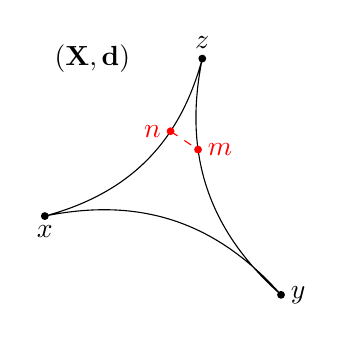
\begin{tikzpicture}[scale=1]
	\draw (0,1) node[fill,circle,inner sep=1pt]{}
	to [bend left] (3,0) node[fill,circle,inner sep=1pt]{} 
	to [bend left] coordinate[pos=.66] (M) (2,3) node[fill,circle,inner sep=1pt]{}
	to [bend left] coordinate[pos=.33] (N) cycle;
	\draw (0,1) node[below]{$x$};
	\draw (3,0) node[right]{$y$};
	\draw (2,3) node[above]{$z$};
	\draw (N) node[fill,circle,inner sep=1pt,color=red]{};
	\draw (N) node[left,color=red]{$n$};
	\draw (M) node[fill,circle,inner sep=1pt,color=red]{};
	\draw (M) node[right,color=red]{$m$};
	\draw[color=red, dashed] (N) -- (M);
	\draw (0,3) node[right]{$\mathbf{(X,d)}$};
	\end{tikzpicture} \hspace{2cm}
	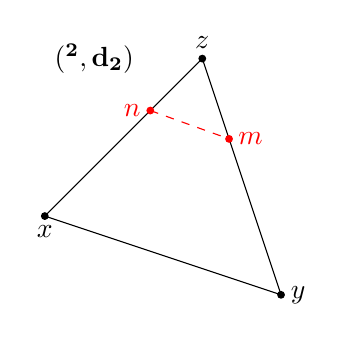
\begin{tikzpicture}[scale=1]
	\draw (0,1) node[fill,circle,inner sep=1pt]{}
	to (3,0) node[fill,circle,inner sep=1pt]{} 
	to coordinate[pos=.66] (M) (2,3) node[fill,circle,inner sep=1pt]{}
	to coordinate[pos=.33] (N) cycle;
	\draw (0,1) node[below]{$\ol{x}$};
	\draw (3,0) node[right]{$\ol{y}$};
	\draw (2,3) node[above]{$\ol{z}$};
	\draw (N) node[fill,circle,inner sep=1pt,color=red]{};
	\draw (N) node[left,color=red]{$\ol{n}$};
	\draw (M) node[fill,circle,inner sep=1pt,color=red]{};
	\draw (M) node[right,color=red,xshift=-.2]{$\ol{m}$};
	\draw[color=red, dashed] (N) -- (M);
	\draw (0,3) node[right]{$\mathbf{(\RR^2,d_2)}$};
	\end{tikzpicture}	
	\caption{Anschaulich gesprochen sind Dreiecke in $\CAT$-Räumen \enquote{mindestens so dünn} wie ihre Vergleichsdreiecke im euklidischen Raum.}
\end{figure}

\begin{bemerkung}
\label{bem:1.8}
	\mbox{} \\[-1.4cm]
	\begin{enumerate}[(i)]
		\item Lokal $\CAT$-Räume heißen auch nichtpositiv gekrümmte oder Alexandrov-Räume.
		\item $\CAT$ steht für \textsc{Cartan-Alexandrov-Topogonov} und Krümmung $\leq 0$.
	\end{enumerate}
\end{bemerkung}

\begin{beispiel}
\label{bsp:1.9}
	\mbox{} \\[-1.4cm]
	\begin{enumerate}[(i)]
		\item Der euklidische Raum $\EE^n$ ist $\CAT$.
		\item $(\RR^2,d_1)$ ist nicht $\CAT$: In der folgenden Abbildung~\ref{abb:1.4} ist $d_1(n,m) = 2$, aber $d_2(\ol{n},\ol{m}) = \sqrt{3}$.
		\begin{figure}[h]
			\centering
			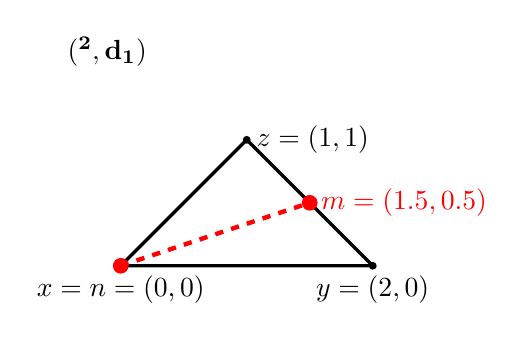
\begin{tikzpicture}[scale=1.6]	
			\draw (-1,0) node[below]{$x = n = (0,0)$};
			\draw (1,0) node[below]{$y = (2,0)$};
			\draw (0,1) node[right]{$z = (1,1)$};
			
			\draw[very thick] (-1,0) node[fill,circle,inner sep=2pt,color=red]{} -- (1,0) node[fill,circle,inner sep=1pt]{} -- coordinate[pos=.5] (M) (0,1) node[fill,circle,inner sep=1pt]{} -- cycle;
			
			\draw (M) node[fill,circle,inner sep=2pt,color=red]{};
			\draw (M) node[right,color=red,xshift=.6]{$m = (1.5,0.5)$};
			\draw[color=red,dashed,ultra thick] (-1,0) -- (M);
			\draw (-1.5,1.7) node[right]{$\mathbf{(\RR^2,d_1)}$};
			\end{tikzpicture} \hspace{1.5cm}
			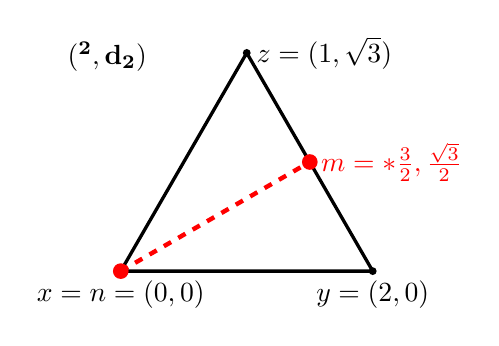
\begin{tikzpicture}[scale=1.6]	
			\draw[very thick] (0,0) node[fill,circle,inner sep=2pt,color=red]{} -- (2,0) node[fill,circle,inner sep=1pt]{} -- coordinate[pos=.5] (M) (1,1.732051) node[fill,circle,inner sep=1pt]{} -- cycle;
			
			\draw (0,0) node[below]{$\ol{x} = \ol{n} =(0,0)$};
			\draw (2,0) node[below]{$\ol{y} = (2,0)$};
			\draw (1,1.732051) node[right]{$\ol{z} = (1,\sqrt{3})$};
			
			\draw (M) node[fill,circle,inner sep=2pt,color=red]{};
			\draw (M) node[right,color=red,xshift=.6]{$\ol{m} = \enbrace*{\frac{3}{2},\frac{\sqrt{3}}{2}}$};
			\draw[color=red,dashed,ultra thick] (0,0) -- (M);
			\draw (-0.5,1.7) node[right]{$\mathbf{(\RR^2,d_2)}$};	
			\end{tikzpicture}
			\caption{Der Raum $(\RR^2,d_1)$ ist nicht $\CAT$.}
			\label{abb:1.4}
		\end{figure}
		\item Hilberträume sind $\CAT$.
		\item Komplemente von Polygonen im $\RR^2$ sind lokal $\CAT$, aber nicht $\CAT$.	
	\end{enumerate}
\end{beispiel}

\begin{beobachtung}
\label{beob:1.10}
	Sei $(X,d)$ ein $\CAT$-Raum.
	Dann ist $X$ eindeutig geodätisch.
\end{beobachtung}

\begin{beweis}
	Seien $\gamma\colon x \geo y$ und $\gamma'\colon x \geo y$ zwei Geodäten von $x$ nach $y$.
	Seien $p$ und $p'$ zwei Punkte auf $\gamma$ und $\gamma'$ mit $d(x,p) = d(x,p')$.
	Das Vergleichsdreieck $\ol{\Delta}$ zum Dreieck
	\[
		\Delta = \Delta\enbrace*{x,p,y\gamma \big|_{[0,d(x,p)]}, \gamma \big|_{[d(x,p),d(x,y)]},\gamma'}
	\]
	ist degeneriert:
	\begin{figure}[h]
		\centering
		\begin{tikzpicture}[scale=1.5,>=Latex]
			\draw (0,0) node[fill,circle,inner sep=1.5pt,color=black]{};
			\draw (3,0) node[fill,circle,inner sep=1.5pt,color=black]{};
			\draw [->,very thick,color=red] (0,0) to [bend left] coordinate[pos=0.3] (P) (3,0);
			\draw [->,very thick,color=blue] (0,0) to [bend right] coordinate[pos=0.3] (Q) (3,0);
			
			\draw (0,0) node[left]{$x$};
			\draw (3,0) node[right]{$y$};
			
			\draw (P) node[fill,circle,inner sep=1.5pt,color=black]{};
			\draw (Q) node[fill,circle,inner sep=1.5pt,color=black]{};
			\draw (P) node[above]{$p$};
			\draw (Q) node[below]{$p'$};
			
			\draw[color=red] (1.5,.5) node[above]{$\gamma$};
			\draw[color=blue] (1.5,-.5) node[below]{$\gamma'$};
		\end{tikzpicture} \hspace{2cm}
		\begin{tikzpicture}[scale=1.5,>=Latex]
		\draw (0,0) node[fill,circle,inner sep=1.5pt,color=black]{};
		\draw (3,0) node[fill,circle,inner sep=1.5pt,color=black]{};
		\draw [->,very thick,color=red] (0,0.01) to coordinate[pos=0.3] (P) (3,0.01);
		\draw [->,very thick,color=blue] (0,-0.01) to  coordinate[pos=0.3] (Q) (3,-0.01);
		
		\draw (0,0) node[left]{$\ol{x}$};
		\draw (3,0) node[right]{$\ol{y}$};
		
		\draw (P) node[fill,circle,inner sep=1.5pt,color=black]{};
		\draw (Q) node[fill,circle,inner sep=1.5pt,color=black]{};
		\draw (P) node[above]{$\ol{p}$};
		\draw (Q) node[below]{$\ol{p'}$};
		
		\draw[color=red] (1.5,.1) node[above]{$\ol{\gamma}$};
		\draw[color=blue] (1.5,-.1) node[below]{$\ol{\gamma'}$};
		\end{tikzpicture}
	\end{figure}
	
	Wegen der $\CAT$-Eigenschaft gilt $d(p,p') \leq d(\ol{p},\ol{p'}) = 0$, also folgt $d(p,p')=0$ und $p = p'$.
\end{beweis}

\begin{definition}[Konvexe Menge]
\label{def:1.11}
	Sei $X$ ein $\CAT$-Raum. Eine nichtleere Teilmenge $C \subseteq X$ heißt \Index{konvex}, wenn zu allen $p,q \in C$ die Geodäte $\gamma \colon p \geo q$ in $C$ liegt.
\end{definition}

Offensichtlich ist $C$ wieder ein $\CAT$-Raum und Durchschnitte konvexer Mengen sind wieder konvex.

\begin{theorem}[{\cite[\hspace{0cm}1A.6]{BridsonHaefliger}}]
\label{th:1.12}
	Sei $\mathcal{M}$ eine einfach zusammenhängende Riemannsche Mannigfaltigkeit nichtpositiver Krümmung. \marginnote{23.10.15 \\ \ [2]}
	Dann ist $\mathcal{M}$ $\CAT$.	
\end{theorem}
\newpage
\begin{satz}
\label{satz:1.13}
	Sei $(V,\Norm{\cdot})$ ein reeller normierter Vektorraum.
	Dann ist $(V,\Norm{\cdot})$ genau dann ein $\CAT$-Raum, wenn $(V,\Norm{\cdot})$ ein Prähilbertraum ist, das heißt es existiert eine symmetrische positiv definite Bilinearform $\sprod{\cdot,\cdot}\colon V \times V \rightarrow \RR$ mit $\Norm{v} = \sqrt{\sprod{v,v}}$ für $v \in V$.
\end{satz}

Für den Beweis brauchen wir eine metrische Charakterisierung von Prähilberträumen:

\vspace*{.5cm}

\begin{minipage}{0.6\textwidth}
	\begin{proposition}[\textsc{von Neumann}, 1935]
		\label{prop:1.14}
		Ein reeller normierter Vektorraum $(V,\Norm{\cdot})$ ist ein Prähilbertraum genau dann, wenn für alle $v,w \in V$ die \Index{Parallelogrammgleichung} gilt:
		\begin{align}
		\Norm{v-w}^2 + \Norm{v+w}^2 = 2 \cdot (\Norm{v}^2 + \Norm{w}^2) \tag{PG} \label{eq:PG}
		\end{align}
	\end{proposition}
\end{minipage}
~
\begin{minipage}{0.35\textwidth}
		\begin{tikzpicture}[scale=1,>=Latex]
		\draw (0,0) node[fill,circle,inner sep=1.5pt]{};
		\draw (1,2) node[fill,circle,inner sep=1.5pt]{};
		\draw (4,1) node[fill,circle,inner sep=1.5pt]{};
		\draw (5,3) node[fill,circle,inner sep=1.5pt]{};
		
		\draw (0,0) node[left]{$0$};
		\draw (1,2) node[left]{$v$};
		\draw (4,1) node[right]{$w$};
		\draw (5,3) node[right]{$v+w$};
		\draw (3.3,1.33) node[rotate=-20]{$\Norm{v-w}$};
		
		\draw [->,thick] (0,0) -- (1,2);
		\draw [->,thick] (0,0) -- (5,3);
		\draw [->,thick] (0,0) -- (4,1);
		\draw [thick,dashed] (1,2) -- (5,3) -- (4,1) -- cycle;
		\end{tikzpicture}
\end{minipage}

\begin{beweis}
	\mbox{} \\[-.85cm]
	\begin{description}
		\item[\bewhin] Seien $u,v \in V$.
		\begin{align*}
			&\Norm{u-v}^2 + \Norm{u+v}^2 \\
			= \  &\sprod{u-v,u-v} + \sprod{u+v,u+v} \\
			= \ &\sprod{u,u} - \sprod{u,v} - \sprod{v,u} + \sprod{v,v} + \sprod{u,u} + \sprod{u,v} + \sprod{v,u} + \sprod{v,v} \\
			= \ &2 \cdot (\sprod{v,v}^2 + \sprod{u,u}^2)
		\end{align*}
		\item[\bewrueck] Definiere:
		\begin{align*}
			b\colon V \times V &\longrightarrow \RR \\
			(u,v) &\longmapsto \frac{1}{4} ( \Norm{u+v}^2 - \Norm{u-v}^2).
		\end{align*} 
		Wir zeigen, dass $b$ ein Skalarprodukt ist: 
		\begin{itemize}
			\item Offensichtlich ist $b$ symmetrisch.
			\item $b$ ist positiv definit, denn für $v \in V$ gilt:
			\begin{align*}
				b(v,v) &= \frac{1}{4} (2\cdot \Norm{v})^2 = \Norm{v}^2 \geq 0 \\
				b(v,v) &= 0 \Leftrightarrow v = 0
			\end{align*}
			\item Sei nun $w \in V$ beliebig. Zu zeigen ist, dass $b(\cdot,w) \colon V \rightarrow \RR$ linear ist. Seien also $u,v \in V$ beliebig, dann gilt:
			\begin{align}
				&b(u+v,w) + b(u-v,w) \\
				\stack{\text{Def}}{=} &\frac{1}{4} (\Norm{\textcolor{blue}{u}+v+\textcolor{blue}{w}}^2 - \Norm{\textcolor{red}{u}+v\textcolor{red}{-w}}^2 + \Norm{\textcolor{blue}{u}-v+\textcolor{blue}{w}}^2 - \Norm{\textcolor{red}{u}-v\textcolor{red}{-w}}^2) \\
				\stack{\eqref{eq:PG}}{=} &\frac{1}{4} (2 \cdot \Norm{u+w}^2 + 2 \cdot \Norm{v}^2 - 2 \cdot \Norm{u-w}^2 - 2\cdot \Norm{v}^2) \\
				\stack{}{=} &\frac{1}{2} (\Norm{u+w}^2 - \Norm{u-w}^2) \\
				\stack{\text{Def}}{=} &2 \cdot b(u,w) \label{eq:1.14.1}
			\end{align}
			Analog erhalten wir
			\begin{equation}
				b(u+v,w) - b(u-v,w) = 2 \cdot b(v,w). \label{eq:1.14.2}
			\end{equation}
			Addition von \eqref{eq:1.14.1} und \eqref{eq:1.14.2} liefert:
			\[ b(u+v,w) = b(u,w) + b(v,w) \]
			Bleibt zu zeigen: Für alle $r \in \RR$ gilt $b(rv,w) = r\cdot b(v,w)$.
			\begin{description}
				\item[1. Fall:] $r=-1$.
				Mit $u = 0$ folgt aus \eqref{eq:1.14.1}:
				\[
					b(v,w) + b(-v,w) = 2 \cdot b(0,w) = 2 \cdot \frac{1}{4} (\Norm{w}^2 - \Norm{-w}^2) = 0
				\]
				und somit $b(-v,w) = -b(v,w)$.
				\item[2. Fall:] $r = n \in \NN$.
				Für $n = 2$ folgt mit $u = v$ aus \eqref{eq:1.14.1}
				\[
					b(2v,w) + \Underbrace{b(0,w)}{=0} = 2 \cdot b(v,w)
				\]
				und weiter induktiv
				\begin{align*}
					b(nv,w) &= b((n-1)v + v,w) = b((n-1)v,w) + b(v,w) \\
					&= (n-1) b(v,w) + b(v,w) = n\cdot b(v,w).
				\end{align*}
				\item[3. Fall:] $r = \frac{1}{n}$ mit $n \in \NN, n \geq 1$.
				Es gilt $\frac{1}{n} \cdot b(nv,w) = b(v,w)$ und damit
				\[
					b\enbrace*{\frac{1}{n} v,w} = \frac{1}{n} \cdot b(n \cdot \frac{1}{n}v,w) = \frac{1}{n} b(v,w)
				\] 
			\end{description}
			Aus allen drei Fällen folgt nun $b(qv,w) = q\cdot b(v,w)$ für alle $q \in \QQ$. Da $\QQ \subseteq \RR$ eine dichte Teilmenge und $b(\cdot,w)$ stetig ist, folgt $b(rv,w) = r \cdot b(v,w)$ für alle $r \in \RR$. \qedhere
		\end{itemize}
	\end{description}
\end{beweis}

\begin{beweis}[Satz~\ref{satz:1.13}]
	\mbox{} \\[-.85cm]
	\begin{description}
		\item[\bewrueck] Sei $\Delta \subseteq (V,\Norm{\cdot}) = \HH$ ein geodätisches Dreieck.
		Dann ist die lineare Hülle $\sprod{\Delta}$ isometrisch isomorph zum $\EE^2$, bzw. zum $\EE^1$ oder zu $\setzero$, falls $\Delta$ degeneriert ist.
		\item[\bewhin] Sei $u,v \in V$ beliebig.
		Zeige, dass für $v,w$ das Parallelogrammgesetz gilt:
		Wir betrachten das Dreieck $\Delta(0,u,v)$ und das Vergleichsdreieck $\ol{\Delta}(0,\ol{u},\ol{v})$.
		Es gilt:
		\begin{align}
			d\enbrace*{\frac{u+v}{2},0} &\makebox[1cm][c]{$\stackrel{\CAT}{\leq}$} d_2\enbrace*{\frac{\ol{u}+\ol{v}}{2},0} \\
			\Rightarrow  d(u+v,0) &\makebox[1cm][c]{$\leq$} d_2(\ol{u}+\ol{v},0) \\
			\Rightarrow \Norm{u+v}^2 \leq \Norm{\ol{u}+\ol{v}}_2^2 &\makebox[1cm][c]{$\stackrel{\eqref{eq:PG}}{=}$} 2 \cdot \Norm{\ol{u}}_2^2 + 2 \cdot \Norm{\ol{v}}_2^2 - \Norm{\ol{u}-\ol{v}}_2^2 \\
			&\makebox[1cm][c]{$\stackrel{\CAT}{=}$} 2 \cdot \Norm{u}^2 + 2 \cdot \Norm{v}^2 - \Norm{u-v}^2 \label{eq:1.13.1}
		\end{align}
		Betrachte das Dreieck $\Delta(0-v,u)$ und das Vergleichsdreieck $\ol{\Delta}(0-\ol{v},\ol{u})$.
		Wir erhalten genauso wie oben die Ungleichung
		\begin{equation}
			\Norm{u-v}^2 \leq 2 \cdot \Norm{u}^2 + 2 \cdot \Norm{v}^2 - \Norm{u+v}^2. \label{eq:1.13.2}
		\end{equation}
		Insgesamt haben wir also:
		\[
			\Norm{u+v}^2 \stackrel{\eqref{eq:1.13.1}}{\leq} 2 \cdot \Norm{u}^2 + 2\cdot \Norm{v}^2 - \Norm{u-v}^2 \stackrel{\eqref{eq:1.13.2}}{\leq} \Norm{u+v}^2 \qedhere
		\]
	\end{description}
\end{beweis}

\begin{erinnerung}[Orthogonale Projektion]
\label{erin:1.15}
	Gegeben sei ein reeller Hilbertraum $\EE^d$ und $U \subseteq \EE^d$ ein Unterraum.
	Sei weiter $v_1,\dots,v_n \in U$ eine Orthonormalbasis von $U$.
	Dann ist \index{orthogonale Projektion}
	\begin{align*}
		\pi_U \colon V &\longrightarrow U \\
		v &\longmapsto \sum_{i=0}^{n} \sprod{v,v_i} \cdot v_i
	\end{align*}
	eine lineare Abbildung und es gilt
	\[
		d(v,\pi_U(v)) = \inf_{u\in U} d(v,u) =: d(v,U)
	\]
	und $v- \pi_U(v) \perp U$.
\end{erinnerung}

\begin{satz}[Projektion auf konvexe Teilmengen]
	Sei $X$ ein $\CAT$-Raum und $C \subseteq X$ konvex und vollständig mit der induzierten Metrik.
	Dann gilt:
	\begin{enumerate}[(i)]
		\item Für alle $x \in X$ existiert genau ein $\pi_C(x) \in C$ mit
		\[
			d(x,\pi_C(x)) = \inf_{p \in C} d(x,p) =: d(x,C).
		\]
		Die Abbildung $\pi_C \colon X \rightarrow C$ heißt die \textbf{(orthogonale) Projektion} auf $C$. \index{orthogonale Projektion}
		\item Ist $y \in [X, \pi_C(x)] = \im(\gamma \colon x \geo \pi_C(x))$, so ist $\pi_C(y) = \pi_C(x)$.
		\item Für alle $x,y \in X$ gilt
		\[
			d(\pi_C(x),\pi_C(y)) \leq d(x,y),
		\]
		das heißt $\pi_C$ ist $1$-Lipschitz. \index{Lipschitz}
	\end{enumerate}
\end{satz}
\newpage
\begin{beweis}
	\mbox{}\\[-.85cm]
	\begin{enumerate}[(i)]
		\item Sei $(y_n)_{n \in \NN} \subseteq C$ eine Folge mit $d(x,y_n) \rightarrow d(x,C) =: D$.
		Zeil ist es zu zeigen, dass $(y_n)_n$ eine Cauchy-Folge ist.
		Da $C$ vollständig ist, ist die Folge $(y_n)_n$ konvergent in $C$ und wir können $\pi_C(x) := \lim\limits_{n \rightarrow \infty} y_n$ definieren.
		
		Zur Eindeutigkeit von $\pi_C(x)$: Angenommen, es existiert ein $\pi_C(x') \in C$ mit $\pi_C(x)' \neq \pi_C(x)$ und $d(x,\pi_C(x)') = d(x,C)$. Betrachte die Folge
		\[
			q_n := \begin{dcases}
				\pi_C(x), & n \text{ gerade} \\
				\pi_C(x)', & n \text{ ungerade}.
			\end{dcases}
		\]
		Dann ist $d(x,q_n) \rightarrow d(x,C)$, aber $(q_n)_n$ ist keine Cauchy-Folge. Widerspruch.
		
		Zur Existenz: Betrachte folgendes Dreieck und Vergleichsdreieck ergänzt zu einem Parallelogramm:
		
		\begin{figure}[h]
			\centering
			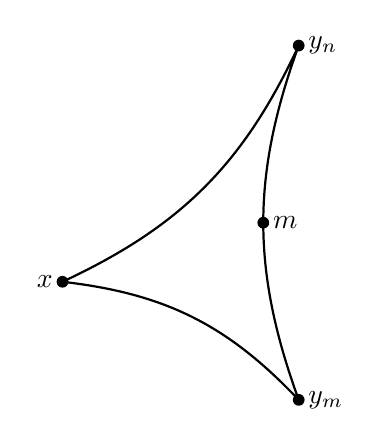
\begin{tikzpicture}[scale=1.5]
				\draw (0,0) node[fill,circle,inner sep=1.5pt]{};
				\draw (2,-1) node[fill,circle,inner sep=1.5pt]{};
				\draw (2,2) node[fill,circle,inner sep=1.5pt]{};
				
				\draw[thick] (0,0) to [bend angle=20, bend left] (2,-1) to [bend angle=20, bend left] coordinate[pos=.5] (M) (2,2) to [bend angle=20, bend left] (0,0);
				
				\draw (0,0) node[left]{$x$};
				\draw (2,-1) node[right]{$y_m$};
				\draw (2,2) node[right]{$y_n$};
				\draw (M) node[fill,circle,inner sep=1.5pt]{};
				\draw (M) node[right]{$m$};
			\end{tikzpicture} \hspace{1cm}
			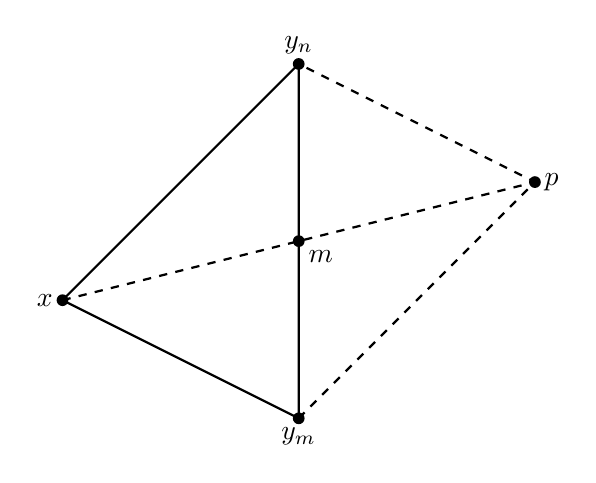
\begin{tikzpicture}[scale=1.5]
				\draw (0,0) node[fill,circle,inner sep=1.5pt]{};
				\draw (2,-1) node[fill,circle,inner sep=1.5pt]{};
				\draw (2,2) node[fill,circle,inner sep=1.5pt]{};
				\draw (4,1) node[fill,circle,inner sep=1.5pt]{};
				
				\draw[thick] (0,0) to (2,-1) to coordinate[pos=.5] (M) (2,2) to (0,0);
				\draw[thick,dashed] (2,-1) -- (4,1) -- (2,2);
				\draw[thick,dashed] (0,0) -- (4,1);
				
				\draw (0,0) node[left]{$\ol{x}$};
				\draw (2,-1) node[below]{$\ol{y_m}$};
				\draw (2,2) node[above]{$\ol{y_n}$};
				\draw (4,1) node[right]{$\ol{p}$};
				\draw (M) node[fill,circle,inner sep=1.5pt]{};
				\draw (M) node[anchor=north west]{$\ol{m}$};
			\end{tikzpicture}
		\end{figure}
		
		Es ist $d(y_n,m) = d(y_m,m) = \frac{1}{2} d(y_n,y_m)$.
		Die Parallelogrammgleichung in $\EE^2$ besagt:
		\[
			d_2(\ol{x},\ol{p})^2 + d_2(\ol{y_n},\ol{y_m})^2 = 2 (d_2(\ol{x},\ol{y_n})^2 + d_2(\ol{x},\ol{y_m})^2)
		\]
		Sei $\varepsilon > 0$. Sei $\delta > 0$ die positive Lösung von $\delta^2 + 2D\delta - \frac{\varepsilon^2}{4} = 0$, das heißt $\varepsilon = 2 \cdot \sqrt{\delta^2+2D\delta}$.
		
		Wähle $n,m$ groß genug, sodass gilt
		\begin{equation}
			\left. \begin{array}{rr}
				d(x,y_n) < D + \delta \\
				d(x,y_m) < D + \delta
			\end{array} \right\}  \forall n,m \geq N. \label{eq:1.16.1}
		\end{equation}
		Aus der $\CAT$-Eigenschaft folgt
		\begin{equation}
			D \leq d(x,m)^2 \leq d_2(\ol{x},\ol{m}). \label{eq:1.16.2}
		\end{equation}
		\newpage
		Damit gilt: 
		\begin{align*}
			d(y_n,y_m)^2 \stack{\CAT}{=} &d_2(\ol{y_n},\ol{y_m}) \\
			\stack{\eqref{eq:PG}}{=} &2 \cdot (d_2(\ol{x},\ol{y_n}) + d_2(\ol{x},\ol{y_m})^2) - d_2(\ol{x},\ol{p})^2 \\
			\stack{}{=} &2 \cdot (d_2(\ol{x},\ol{y_n}) + d_2(\ol{x},\ol{y_m})^2) - 4\cdot d_2(\ol{x},\ol{m})^2 \\
			\stack{\eqref{eq:1.16.2}}{\leq} &2 \cdot (d_2(\ol{x},\ol{y_n}) + d_2(\ol{x},\ol{y_m})^2) - 4D^2 \\
			\stack{\eqref{eq:1.16.1}}{\leq}  &2 \cdot (2 \cdot (D+\delta)^2) - 4D^2 \\
			\stack{}{=} &4\cdot (2D\delta + \delta^2)
		\end{align*}
		Somit folgt $d(y_n,y_m) \leq 2 \cdot \sqrt{2D\delta + \delta^2} = \varepsilon$ für $n,m \geq N$.
		Also ist $(y_n)_n$ eine Cauchy-Folge und wir setzen $\pi_C(x) := \lim_{n \rightarrow \infty} y_n$. \qedhere
	\end{enumerate}
\end{beweis}

\cleardoubleoddemptypage